\documentclass[mathserif, 10pt]{beamer}
\usepackage[utf8]{inputenc}
\usepackage{amsmath, amsfonts}
\usepackage{appendixnumberbeamer}


\title[Using ML techniques in phenomenological studies in flavour physics]{Using Machine Learning techniques in\\ phenomenological studies in flavour physics}
\subtitle{Jorge Alda,\\ Universidad de Zaragoza/CAPA \hspace{4em} \texttt{jalda@unizar.es} }
\author[Jorge Alda]{Based on \textbf{JA}, J. Guasch, S. Peñaranda \\
arXiv:2109.07405 [hep-ph]}

\date[Unizar Seminar]{Unizar Seminar, 20th January 2022}



\usetheme{Zaragoza}
\usecolortheme{Unizar}
\titlepagelogoA{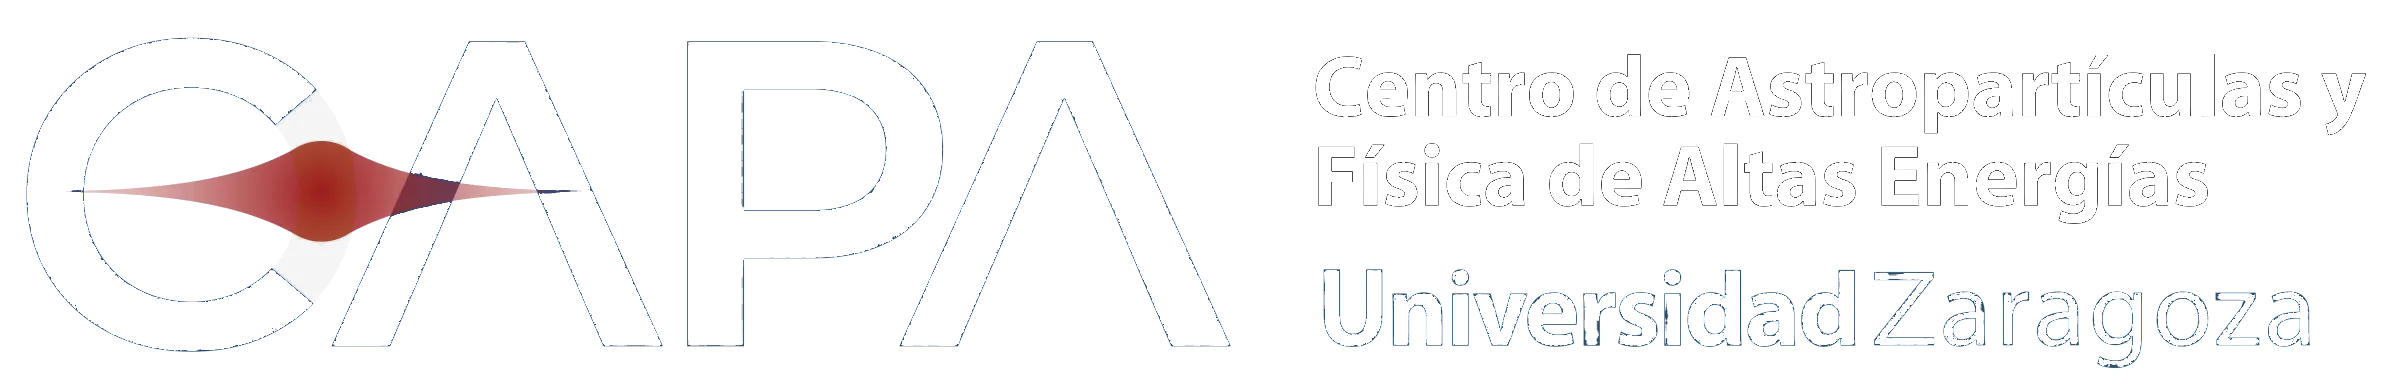
\includegraphics[width=6cm]{logos/CAPA.png}}
\titlepagelogoB{
\includegraphics[width=4cm]{logos/dftuz2.png}}


\newcommand\colorcite[1]{{\scriptsize\color{blue}#1}}

\begin{document}
\begin{frame}[noframenumbering,plain]
\titlepage
\end{frame}

\begin{frame}
    \frametitle{$B$ anomalies}

    Experimental results for the decays of $B$ mesons that don't conform with the SM predictions.

    ~

    In particular, these anomalies show hints of violation of the Leptonic Flavour Universality (LFU).

\end{frame}

\begin{frame}
    \frametitle{$B$ anomalies}

    Flavour-changing neutral currents $b \to s \ell^+ \ell^-$, with $\ell = e, \mu$.
    \begin{itemize}
        \item Universality ratios $R_{K^{(*)}}$
              $$R_{K^{(*)}} = \frac{\mathrm{BR}(B\to K^{(*)}\mu^+ \mu^-)}{\mathrm{BR}(B\to K^{(*)}e^+ e^-)}\,, $$
              In the SM, theoretically clean, and $R_{K^{(*)}}=1$.\\
              LHCb measurements\footnote{R. Aaij \textit{et al.} (LHCb) arXiv:2103.11769, arXiv:1705.05802}:
              \begin{itemize}
                  \item $R_{K^+} = 0.846^{+0.042}_{-0.039}{}^{+0.013}_{-0.012}$,
                  \item $R_{K^{*0}} = 0.685^{+0.113}_{-0.069}\pm0.047$. ($3.1\,\sigma$ tension)
              \end{itemize}
        \item Angular observables for $B\to K^* \ell^+\ell^-$: $P'_4$, $P'_5\ldots$
        \item Also $B_s \to \phi \mu^+ \mu^-$ decays.
    \end{itemize}

\end{frame}

\begin{frame}
    \frametitle{$B$ anomalies}
    Flavour-changing charged currents $b\to c \ell \nu$, with $\ell = e/\mu, \tau$.
    \begin{columns}
        \begin{column}{0.55\textwidth}

            \begin{itemize}
                \item Universality ratios $R_{D^{(*)}}$
                      $$R_{D^{(*)}} = \frac{\mathrm{BR}(B\to D^{(*)}\tau \nu)}{\mathrm{BR}(B\to D^{(*)}\ell \nu)}\,, $$
                      $$R_D = 0.340 \pm 0.027 \pm 0.013\,,$$
                      $$R_{D^*} = 0.295 \pm 0.011 \pm 0.008\,.$$
                      Combined tension of $3.08\,\sigma$.\footnotemark[1]
                \item Longitudinal polarization of $D^*$.
                \item Also $B_c \to J/\psi \ell\nu$ decays.
            \end{itemize}

        \end{column}
        \begin{column}{0.5\textwidth}
            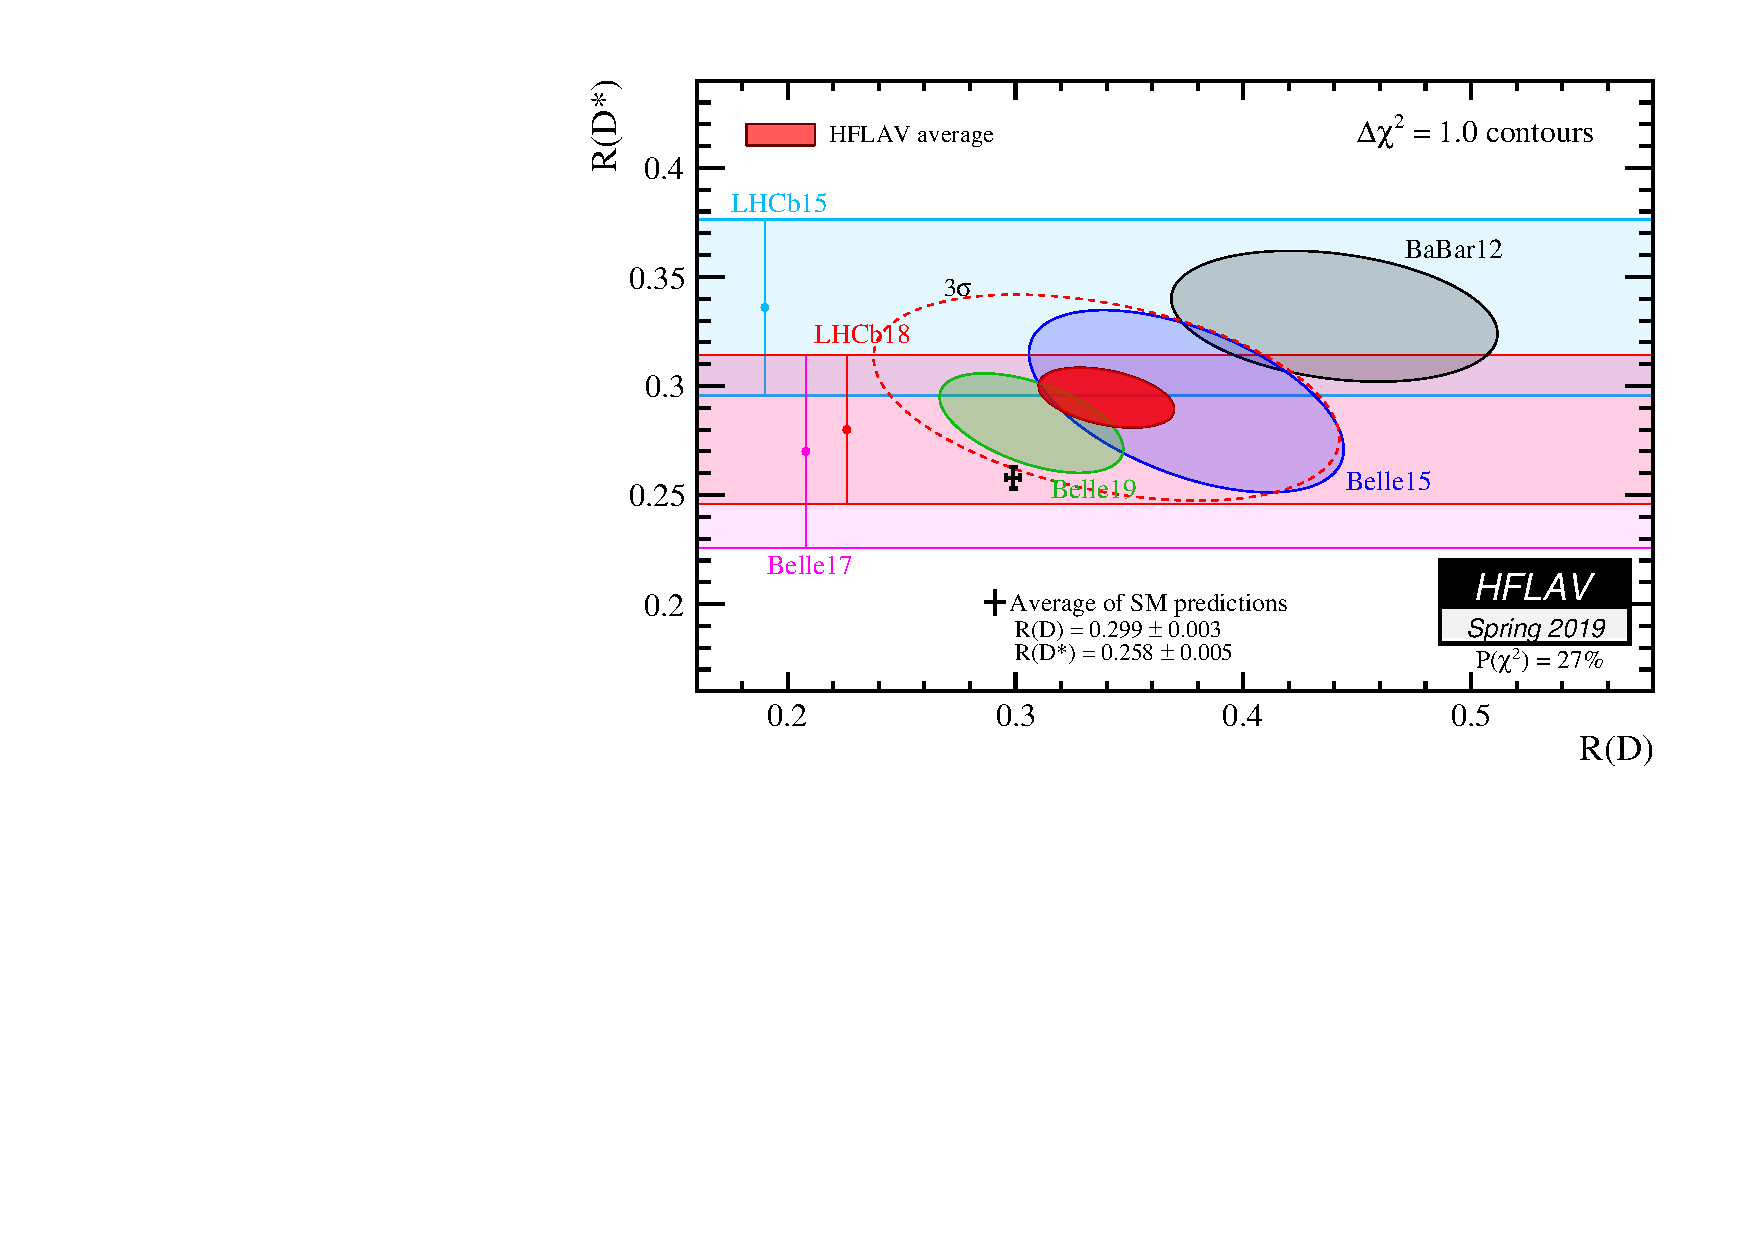
\includegraphics[width=\columnwidth]{figures/rdrds_spring2019.pdf}
        \end{column}
    \end{columns}
    \footnotetext[1]{Y. S. Ahmis \textit{et al.} (HFLAV) arXiv:1909.12524}
\end{frame}

\begin{frame}
    \frametitle{Effective Field Theories}

    Effective Field Theories (EFTs) describe deviations from the SM in a model-independent way, using effective operators of dim $>4$ and their corresponding Wilson coefficients.

    ~

    At energies $\Lambda$ above the electroweak scale, the dim-6 SMEFT (2499 operators)\footnote[1]{B.~Grzadkowski, M.~Iskrzynski, M.~Misiak and J.~Rosiek. arXiv:1008.4884}

    $$\mathcal{L} = \mathcal{L}_\mathrm{SM} + \frac{1}{\Lambda^2}\sum C_i O_i\,.$$

    We will focus on the following operators at $\Lambda = 1\,\mathrm{TeV}$:

    $$O_{\ell q(1)}^{ijkl} = (\bar{\ell}_i \gamma_\mu \ell_j)(\bar{q}_k \gamma^\mu  q_l),\qquad\qquad O_{\ell q(3)}^{ijkl}= (\bar{\ell}_i \gamma_\mu \tau^I \ell_j)(\bar{q}_k \gamma^\mu \tau^I q_l)\,.$$

\end{frame}

\begin{frame}

    \frametitle{Effective Field Theories}
    The $B$ anomalies are defined at $\mu=m_b$, we need to integrate the heavy SM particles. We obtain the WET\@:

    ~

    \begin{itemize}
        \item $\left.\begin{matrix}
                      O_9^\ell = (\bar{s}_L \gamma_\alpha b_L)(\bar{e}_\ell \gamma^\alpha e_\ell) \\
                      O_{10}^\ell = (\bar{s}_L \gamma_\alpha b_L)(\bar{e}_\ell \gamma^\alpha \gamma_5 e_\ell)
                  \end{matrix}\right\} \qquad \Longrightarrow \qquad R_{K^{(*)}}$. % chktex 21

              ~

        \item $O_{VL}^\ell = (\bar{c}_L \gamma_\alpha b_L)(\bar{e}_{\ell\,L} \gamma^\alpha \nu_\ell) \qquad\Longrightarrow\qquad R_{D^{(*)}}$.

              ~

        \item $O_\nu^\ell = (\bar{s}_L \gamma_\alpha b_L)(\bar{\nu}_\ell (1-\gamma_5) \nu_\ell) \qquad\Longrightarrow \qquad \mathrm{BR}(B\to K^{(*)}\nu\overline{\nu})$.
    \end{itemize}



\end{frame}

\begin{frame}
    \frametitle{Effective Field Theories}
    Translating between the two EFTs: 1-loop RG running $\Lambda \to \mu_\mathrm{EW}$ + matching:
    \begin{itemize}
        \item {\small $C_9^\ell \approx \frac{\sqrt{2}}{V_{tb}V_{ts}^* G_F \Lambda^2}\left[ \frac{2\pi^2}{e^2}(C_{\ell q(1)}^{\ell\ell23}+C_{\ell q(3)}^{\ell\ell23}) + \textcolor{blue}{\frac{\log(m_b/\Lambda)}{3}(C_{\ell q(1)}^{3323}+C_{\ell q(3)}^{3323})}\right]\, $.}
        \item {\small $C_{10}^\ell \approx \frac{-\sqrt{2}}{V_{tb}V_{ts}^* G_F \Lambda^2} \frac{2\pi^2}{e^2}(C_{\ell q(1)}^{\ell\ell23}+C_{\ell q(3)}^{\ell\ell23}) \, $.}
\item {\small $C_{VL}^\ell \approx \frac{-1}{\sqrt{2}G_F\Lambda^2}\left(C_{\ell q(3)}^{\ell\ell33}+ \frac{V_{cs}}{V_{cb}}C_{\ell q(3)}^{\ell\ell 23}\right)$\,.}
        \item {\small $C_\nu^\ell \approx \frac{\sqrt{2}}{e^2 V_{tb}V_{ts}^* G_F \Lambda^2}\left[2\pi^2(C_{\ell q(1)}^{\ell\ell 23}-C_{\ell q(3)}^{\ell\ell 23})+\textcolor{blue}{\frac{2{g'}^2}{3}\log(m_b/\Lambda)C_{\ell q(3)}^{\ell\ell 23}}\right]\,$.}
    \end{itemize}

\textcolor{blue}{Loop-level corrections} break the relation $C_9^\ell = -C_{10}^\ell$.
\blankfootnote{\textbf{J.A.}, J. Guasch and S. Peñaranda. arXiv:2109.07404}
\end{frame}

\begin{frame}
    \frametitle{Effective Field Theories}

    Our setting: in the interaction basis, NP only affects the third generation,\footnote[1]{F.~Feruglio, P.~Paradisi and A.~Pattori. arXiv:1705.00929}
    $$C_1 = C_{\ell q(1)}^{3333}\,,\qquad\qquad C_3 = C_{\ell q(3)}^{3333}\,.$$
    We have to rotate to the mass basis, using rotation matrices $\lambda^q$ and $\lambda^\ell$,
    $$C_{\ell q(1)}^{ijkl} = C_1 \lambda_\ell^{ij}\lambda_q^{kl}\,\qquad\qquad C_{\ell q(3)}^{ijkl} = C_3 \lambda_\ell^{ij}\lambda_q^{kl}\,. $$
    The rotation matrices must be hermitian, idempotent and with $\mathrm{tr}\lambda =1$. Parameterized as
    $$ \lambda = \frac{1}{1+|\alpha|^2+|\beta|^2}\begin{pmatrix}
            |\alpha|^2 & \alpha \beta^* & \alpha \\ \alpha^* \beta & |\beta|^2 & \beta \\ \alpha^* & \beta^* & 1
        \end{pmatrix}\,. $$
    We will fix $C_1 = C_3$ to avoid large deviations in the $B\to K^{(*)}\nu\overline{\nu}$ decays.
\end{frame}

\begin{frame}
    \frametitle{Global fits}
    \begin{itemize}
        \item The structure of the $\lambda$ matrices creates Lepton Flavour Violating effects through $\lambda_\ell^{ij}\, (i\neq j)$.
        \item RG evolution causes mixing between effective operators:
              \begin{itemize}
                  \item For example, $O_{\ell q(1)}$ mixes with $O_{\varphi \ell(1)} = (\varphi^\dagger i \overleftrightarrow D_{\mu} \varphi)(\bar{\ell} \gamma^\mu \ell )$ that modifies the $Z\ell^+\ell^-$ couplings.
              \end{itemize}
    \end{itemize}

    ~

    We need to consider the effects of the New Physics in a wide range of experimentally-measured observables: Global Fits.


\end{frame}

\begin{frame}
    \frametitle{Global fits}

    Tools used for the global fits (in \texttt{python3}):
    \begin{itemize}
        \item \texttt{wilson}\footnote[1]{J.~Aebischer, J.~Kumar and D.~M.~Straub. arXiv:1804.05033}: RG evolution and mixing of the Wilson coefficients.
        \item \texttt{flavio}\footnote[2]{D.~M.~Straub. arXiv:1810.08132}: Calculation of observables in EFTs and database of experimental measurements.
        \item \texttt{smelli}\footnote[3]{J.~Aebischer, J.~Kumar, P.~Stangl and D.~M.~Straub. arXiv:1810.07698}: Global likelihood function:
              {\small$$\Delta \log L = -\frac{1}{2}\Delta\chi^2 = -\frac{1}{2}\sum_{i,j} [\mathcal{O}_i^\mathrm{exp} - \mathcal{O}_i(\vec{C})] (\mathcal{C}^\mathrm{th}+\mathcal{C}^\mathrm{exp})^{-1}_{ij} [\mathcal{O}_j^\mathrm{exp} - \mathcal{O}_j(\vec{C})]\,. $$} % chktex 35
    \end{itemize}

\end{frame}

\begin{frame}
    \frametitle{Global fits}
    We perform global fits including $b\to s \ell^+\ell^-$ and
    $b\to c\ell\nu$ observables, and also electroweak precision tests,
    nuclear precision observables (superallowed $\beta$ decays) and Leptonic Flavour Violating observables.

    ~

    We consider two different scenarios:
    \begin{itemize}
        \item \textbf{Scenario I:} Mixing to first generation $\alpha$ are negligible\footnote[1]{F.~Feruglio, P.~Paradisi and A.~Pattori. arXiv:1705.00929}.
        \item \textbf{Scenario II:} Mixing to first and second generations\footnote[2]{\textbf{J.A.}, J. Guasch and S. Peñaranda. arXiv:2109.07404}.
    \end{itemize}
    \begin{center}\small
        \begin{tabular}{|c|c|c|}\hline
             & Scenario I & Scenario II \\\hline
            $C$ & $-0.13 \pm 0.05$ & $-0.13 \pm 0.08$             \\\hline
            $\alpha^\ell$ & & $\pm (0.07^{+0.04}_{-0.07})$ \\\hline
            $\beta^\ell$  & $0 \pm 0.025$ & $0 \pm 0.025$ \\\hline
            $\alpha^q$ & & $-0.05^{+0.12}_{-0.07}$ \\\hline
            $\beta^q$ & $0.8^{+2.0}_{-0.5}$ & $0.73^{+2.8}_{-0.6}$ \\\hline
            $\Delta \chi^2_\mathrm{SM}$ & $40.32$ & $57.06$ \\\hline
            SM Pull & $5.75\,\sigma$ & $6.57\,\sigma$               \\\hline
        \end{tabular}
    \end{center}
\end{frame}

\begin{frame}
    \frametitle{Global fits: Results}
    Regions allowed at $1~\sigma$:
    \begin{center}
        \begin{tabular}{cc}
            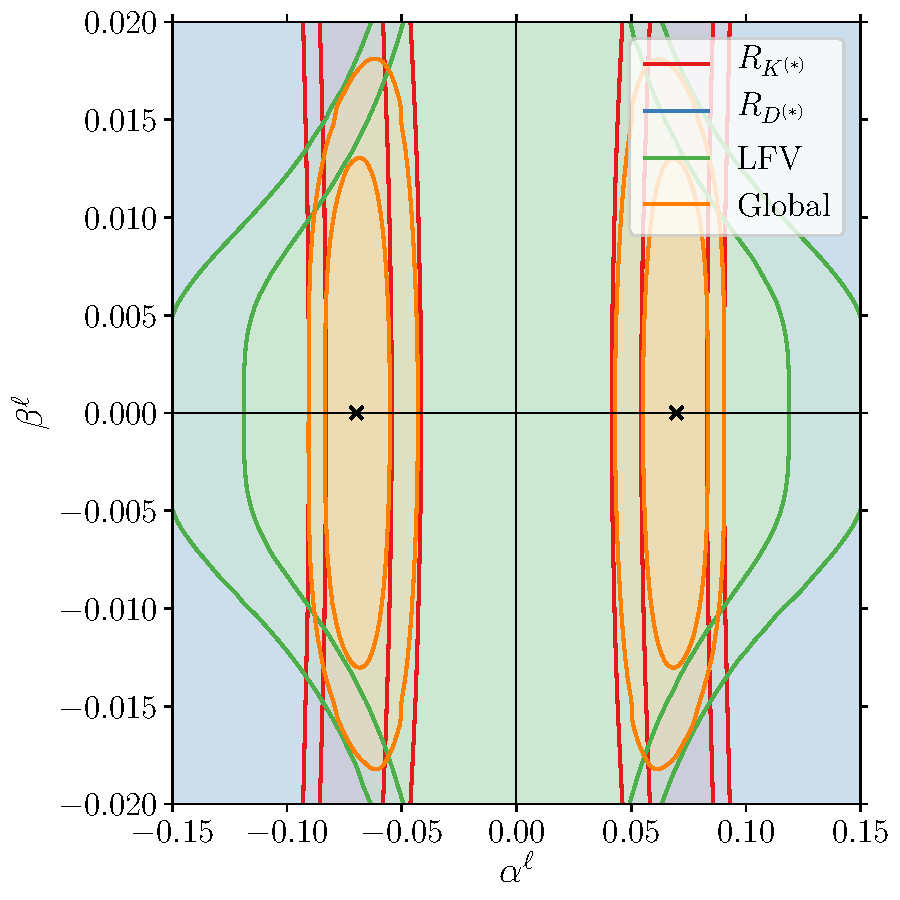
\includegraphics[width=0.4\textwidth]{figures/alphabeta_l.pdf} & 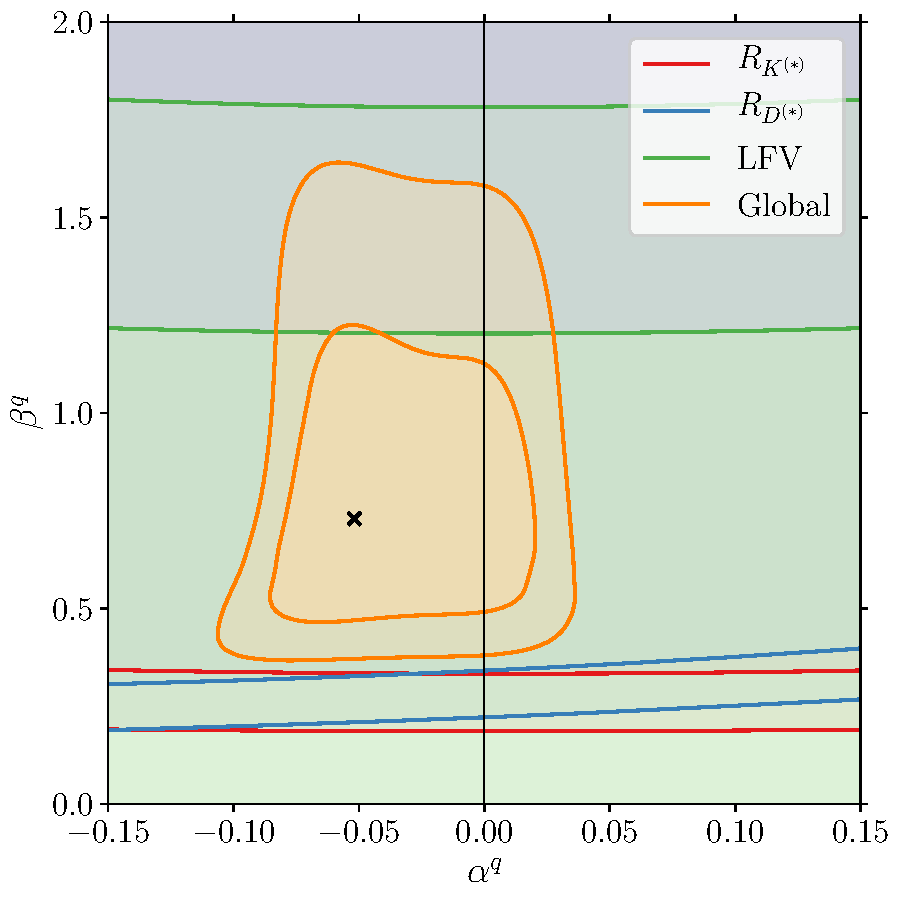
\includegraphics[width=0.4\textwidth]{figures/alphabeta_q.pdf}
        \end{tabular}
    \end{center}
    \begin{itemize}
        \item $\alpha^\ell$ is constrained by $R_{K^{(*)}}$.
        \item $\beta^\ell$ is constrianed by LFV observables.
    \end{itemize}
    \blankfootnote{\textbf{J.A.}, J. Guasch and S. Peñaranda. arXiv:2109.07404}
\end{frame}

\begin{frame}
    \frametitle{Global fits: Results}

    \begin{center}
        \begin{tabular}{lc}
            $R_{K^{(*)}} = \frac{\mathrm{BR}(B\to K^{(*)}\mu^+ \mu^-)}{\mathrm{BR}(B\to K^{(*)}e^+ e^-)}$ & $R_{D^{(*)}} = \frac{\mathrm{BR}(B\to D^{(*)}\tau \nu)}{\mathrm{BR}(B\to D^{(*)}\ell \nu)}$ \\
            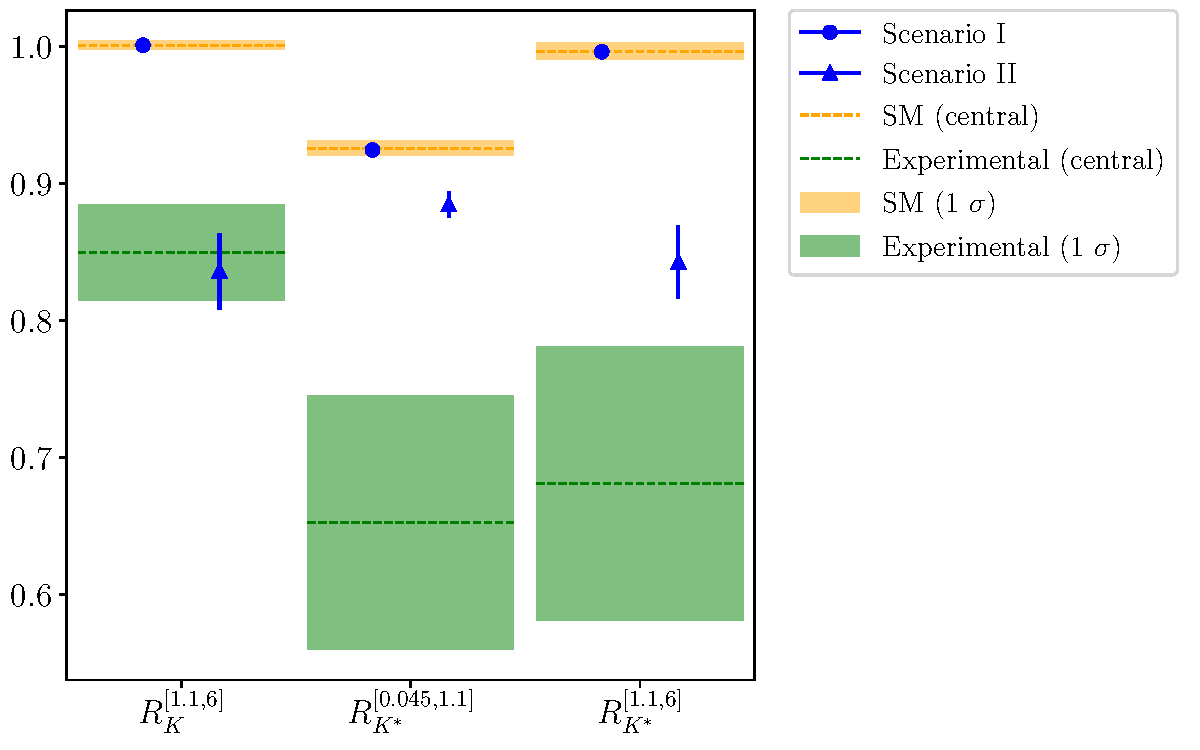
\includegraphics[width=0.55\textwidth]{figures/rotRKplot.pdf} &
            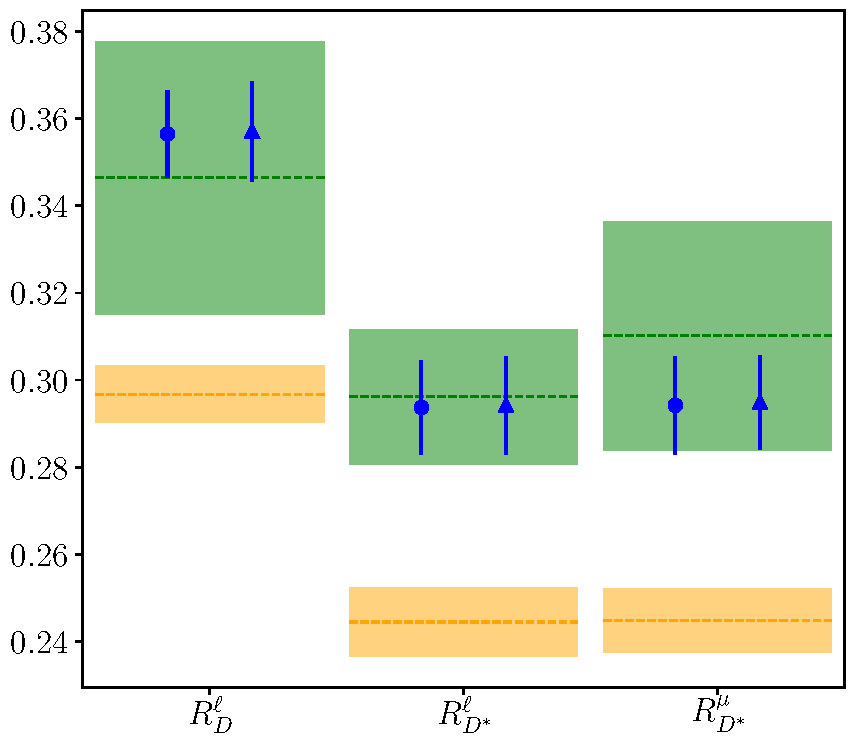
\includegraphics[width=0.4\textwidth]{figures/rotRDplot.pdf}
        \end{tabular}
    \end{center}
    $R_{K^{(*)}}$ requires mixing with the first generation ($\alpha^\ell$):
    \begin{align*}
        C_9^e   & = -C_{10}^e + C_9^\mathrm{loop} = -0.32\,, \qquad\qquad                 &  & C_{10}^e =-0.36\,,             \\
        C_9^\mu & = {\color{gray}-C_{10}^\mu} + C_9^\mathrm{loop} = -0.67\,, \qquad\qquad &  & {\color{gray}C_{10}^\mu =0}\,.
    \end{align*}
    \blankfootnote{\textbf{J.A.}, J. Guasch and S. Peñaranda. arXiv:2109.07404}
\end{frame}

\begin{frame}
    \frametitle{Exploring the likelihood function}

    \begin{itemize}
        \item We would like to explore the properties of the likelihood function around the best fit point.
        \item {\bf Problem:} At each point $(C, \alpha^\ell, \beta^\ell, \alpha^q, \beta^q)$ requires the calculation of 471 observables, many of them need numerical integration.
        \item In a previous work\footnote[1]{\textbf{J.A.}, J.~Guasch and S.~Pe\~naranda. arXiv:2012.14799}, we used the Hessian approximation,
        $$\Delta\log L (\vec{C}) \approx \Delta\log L_\mathrm{bf} + \vec{C}^T \mathbb{H} \vec{C}\,.$$
        \item Doesn't work in this case because of non-linear relation between fit parameters and Wilson coefficients.
        \item {\bf Idea:} Teach a machine to approximate $\log L(\vec{C})$.
    \end{itemize}

\end{frame}

\begin{frame}
    \frametitle{xgboost}

    Decision tree
    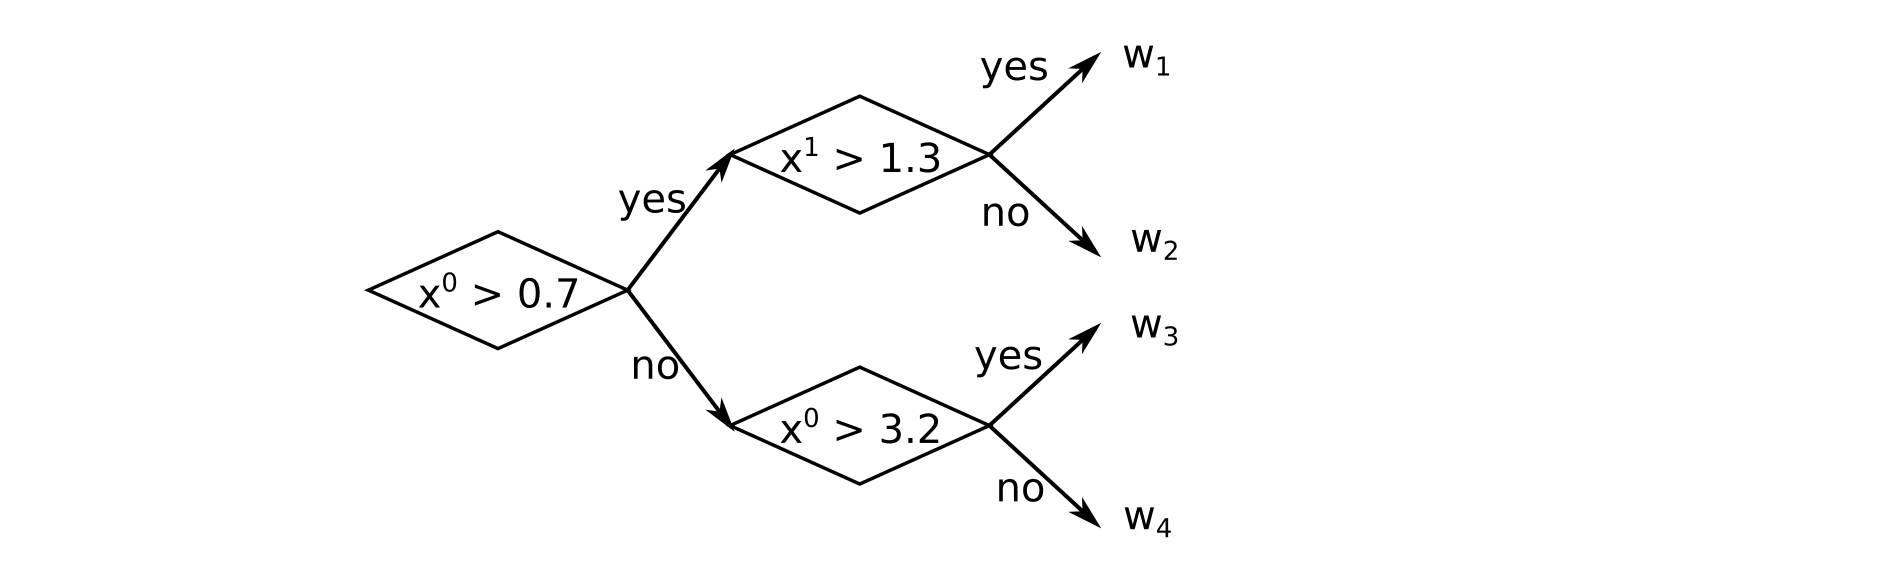
\includegraphics[width=\textwidth]{figures/dectree.png}

    \invisible{A regression tree $k$ defines a function $f_k(x)$. We use an ensemble of trees $F$ for the prediction: $$\phi(x) = \sum_{k\in F} f_k(x)\,.$$}
\end{frame}

\begin{frame}
    \frametitle{xgboost}

    Regression tree
    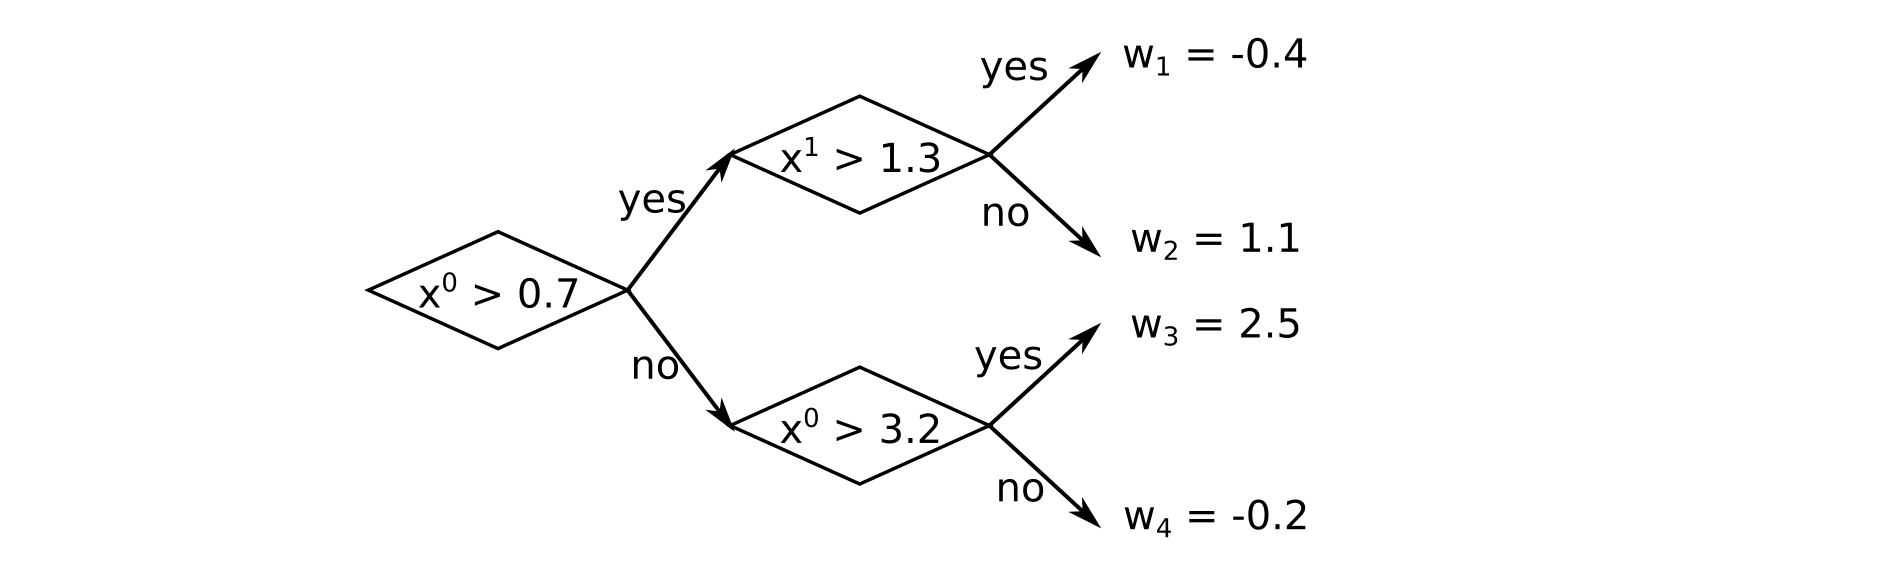
\includegraphics[width=\textwidth]{figures/regtree_nof.png}

    \invisible{A regression tree $k$ defines a function $f_k(x)$. We use an ensemble of trees $F$ for the prediction: $$\phi(x) = \sum_{k\in F} f_k(x)\,.$$}
\end{frame}

\begin{frame}
    \frametitle{xgboost}

    Regression tree
    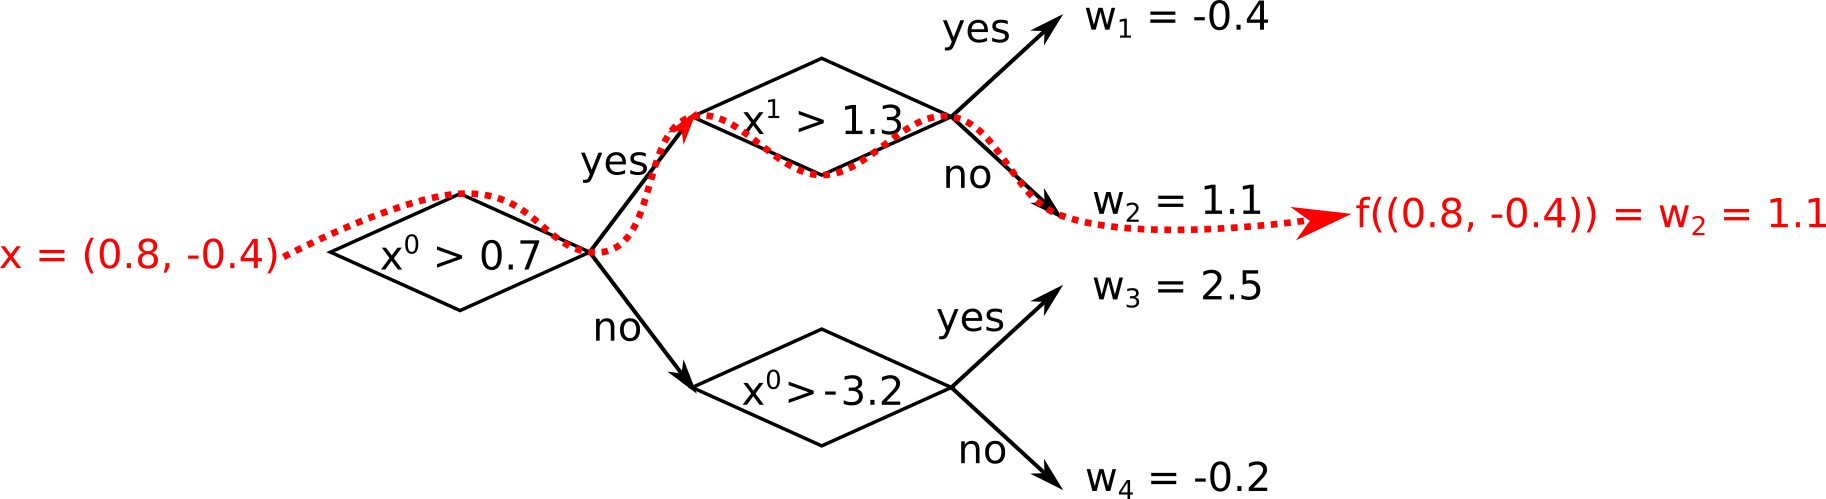
\includegraphics[width=\textwidth]{figures/regtree.png}

    A regression tree $k$ defines a function $f_k(x)$. We use an ensemble of trees $F$ for the prediction: $$\phi(x) = \sum_{k\in F} f_k(x)\,.$$
\end{frame}

\begin{frame}
    \frametitle{xgboost}

    Extreme Gradient Boosting (xgboost)\footnote[1]{T.~Chen and C.~Guestrin. arXiv:1603.02754}.

    ~

    We have a dataset $\{(x_i, y_i)\}$ with $x_i \in X (\sim\mathbb{R}^n)$ and $y_i \in \mathbb{R}$, and want to find $\phi(x)$ so $\phi(x_i)\approx y_i$. Defining the regularized objective
    $$\mathcal{L}[\phi] = \sum_i \ell(\phi(x_i), y_i) + \sum_k \Omega(f_k)\,. $$
\begin{itemize}
    \item $\ell(\tilde{y}_i, y_i)$ is the loss function.
    \item $\Omega(f_k)$ penalizes the complexity of the trees.
\end{itemize}
The objective is optimized iteratively:
\begin{itemize}
    \item The algorithm starts with one tree with a single leaf.
    \item At each step, one new tree with one more leaf is added to the ensemble (splitting).
    \item To prevent overfitting, the weights of the newly added leaf is multiplied by $\eta < 1$ (shrinkage).
\end{itemize}
\end{frame}

\begin{frame}
    \frametitle{Machine Learning training}

    \begin{columns}
        \begin{column}{0.5\textwidth}
            Data sample consisting of
            \begin{itemize}
                \item 5000 points re-used from likelihood plots.
                \item 5000 random points.
                \item Split in 75\% training set, 25\% validation set.
            \end{itemize}
            Results of the training:
            \begin{itemize}
                \item Pearson regression coefficient $r=0.971$.
                \item Mean Absolute Error $0.655$.
            \end{itemize}
        \end{column}
        \begin{column}{0.5\textwidth}
            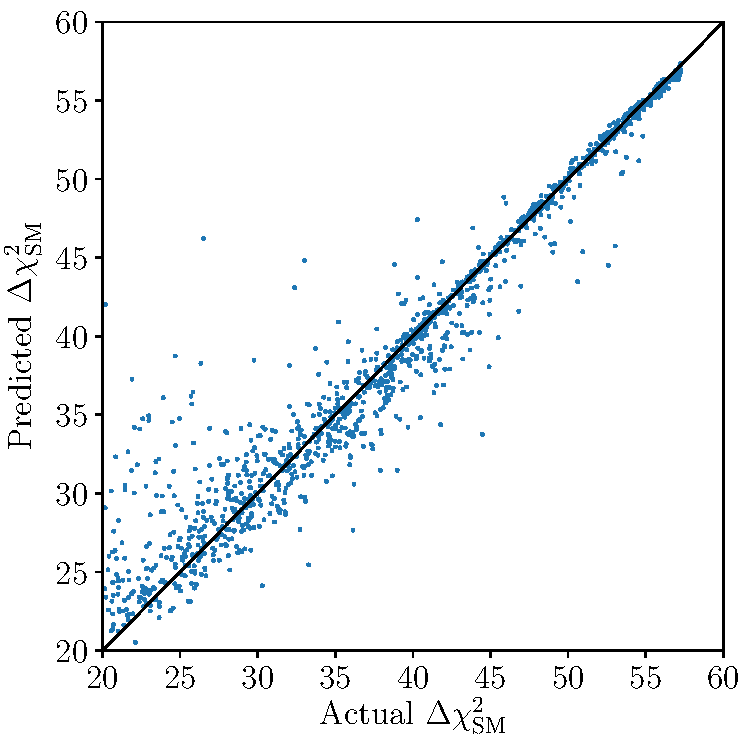
\includegraphics[width=\columnwidth]{figures/regression_xgb.pdf}
        \end{column}
    \end{columns}
    \blankfootnote{\textbf{J.A.}, J. Guasch and S. Peñaranda. arXiv:2109.07404}

\end{frame}

\begin{frame}
    \frametitle{Machine-Learning Montecarlo}
    \begin{columns}
        \begin{column}{0.5\textwidth}
            We want to generate a sample of points distributed according to the $\chi^2$ of the fit.

            We generate random points, that are accepted if
            $$\log \tilde{L}(\vec{C}) = \log L_\mathrm{bf} + \log u\,,$$
            with $u$ a random number from the uniform distribution in $[0,1)$. % chktex 9
        \end{column}
        \begin{column}{0.5\textwidth}
            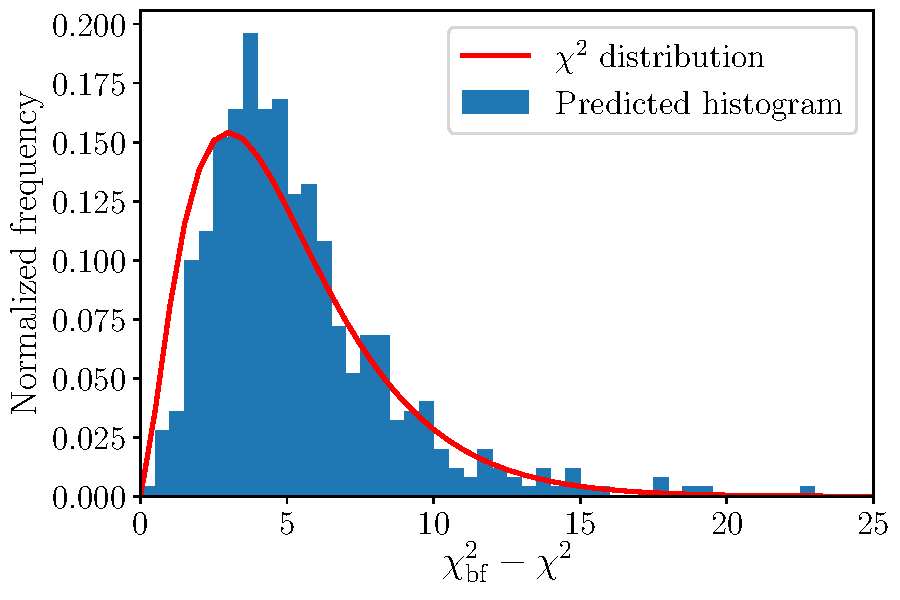
\includegraphics[width=\columnwidth]{figures/hist_xgb.pdf}
        \end{column}
    \end{columns}
    
    ~

    We use the trained model $\log\tilde{L}(\vec{C})$ to compute an approximation of the likelihood function.
    \blankfootnote{\textbf{J.A.}, J. Guasch and S. Peñaranda. arXiv:2109.07404}

\end{frame}

\begin{frame}
    \frametitle{SHAP values}

    Measure of the importance of each parameter in the Machine Learning prediction for a single datapoint\footnote[1]{S. Lundberg, S. Lee. arXiv:1705.07874}. Based on game theory (Lloyd Shapley, Nobel Prize in Economics '12).


    \begin{itemize}
        \item \textbf{Local accuracy:} The sum of all SHAP values (plus a constant) is the ML prediction.
        \item \textbf{Missingness:} If some parameter is missing, its SHAP value is zero.
        \item \textbf{Consistency:} If the model is changed so one parameter has a larger impact, its SHAP value will increase.
    \end{itemize}


\end{frame}

\begin{frame}
    \frametitle{SHAP values}
    We train $2^n$ simplified models

    \begin{columns}
        \begin{column}{0.5\textwidth}
            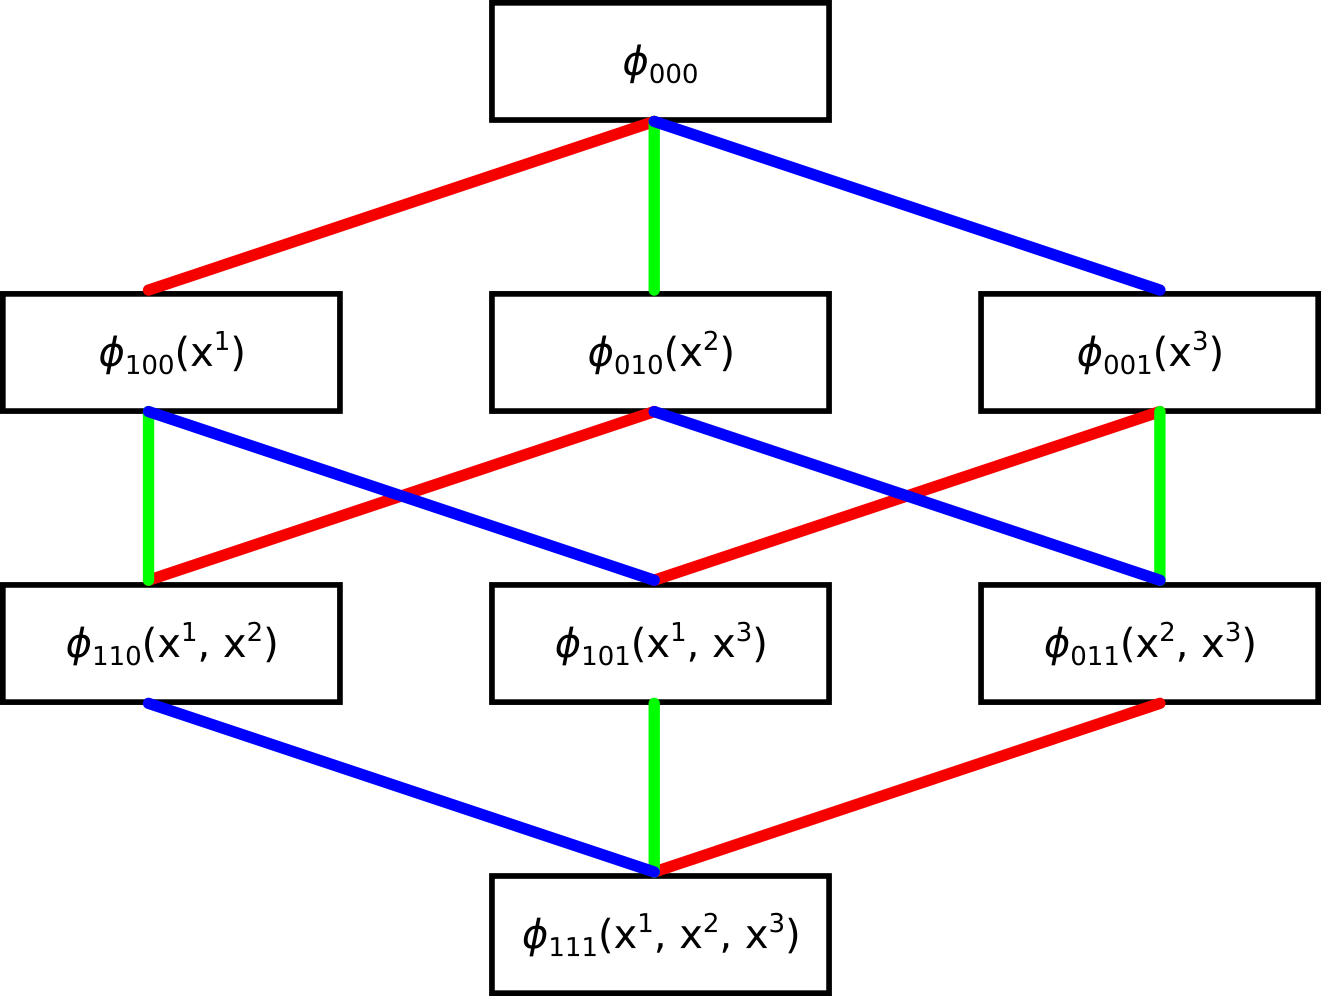
\includegraphics[width=\columnwidth]{figures/shapgraph.png}
        \end{column}
        \begin{column}{0.5\textwidth}
            \begin{itemize}
                \item Marginal contributions {\color{red} when adding $x^1$}: $\phi_{100}-\phi_{000}$, $\phi_{110}-\phi_{010}$, $\phi_{101}-\phi_{001}$, $\phi_{111} - \phi_{011}$.
                \item SHAP value {\color{red}for $x^1$} is a weighted average of all its marginal contributions.
                \item $\phi_{000}$ is the constant value. 
            \end{itemize}
        \end{column}
    \end{columns}
    
    Efficient implementation (poly time) for tree-based Machine Learning models.\footnote[1]{S. Lundberg, G. Erion, S. Lee. arXiv:1802.03888}

\end{frame}

\begin{frame}
    \frametitle{SHAP values: results}

    The mixing \(\beta^q\) to the second quark generation and $\alpha^\ell$ to the first lepton generation are in general the most important features.
    \begin{center}
        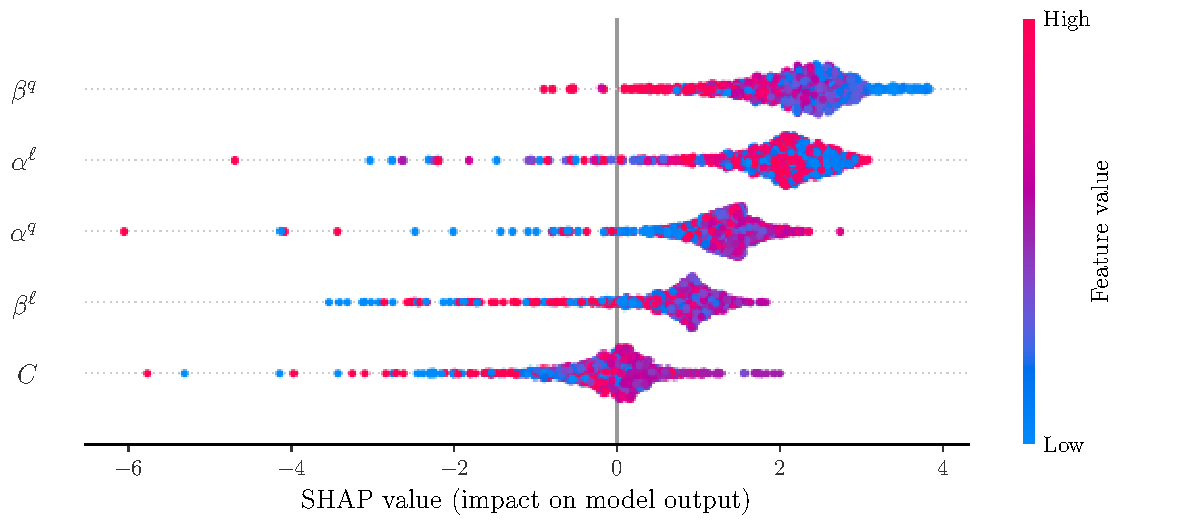
\includegraphics[width=0.8\textwidth]{figures/SHAP_summary.pdf}
    \end{center}
    
    For the best fit point, the value of $C$ is also important:
    \begin{center}
        \begin{tabular}{|*{8}{c|}}\hline
        Base & \multicolumn{5}{c|}{SHAP value for} & Final & Actual \\ \cline{2-6}
        value & $C$ & $\alpha^\ell$ & $\beta^\ell$ & $\alpha^q$ & $\beta^q$ & prediction & $\log L$ \\\hline
        39.43 & 3.293 & 4.056 & 1.993 & 2.671 & 4.086 & 55.537 & 57.06 \\\hline
        \end{tabular}
        \end{center}
        \blankfootnote{\textbf{J.A.}, J. Guasch and S. Peñaranda. arXiv:2109.07404}

\end{frame}

\begin{frame}
    \frametitle{SHAP values: results}
    SHAP importances reproduce the dependence of the $-\log L$:
    \begin{center}
        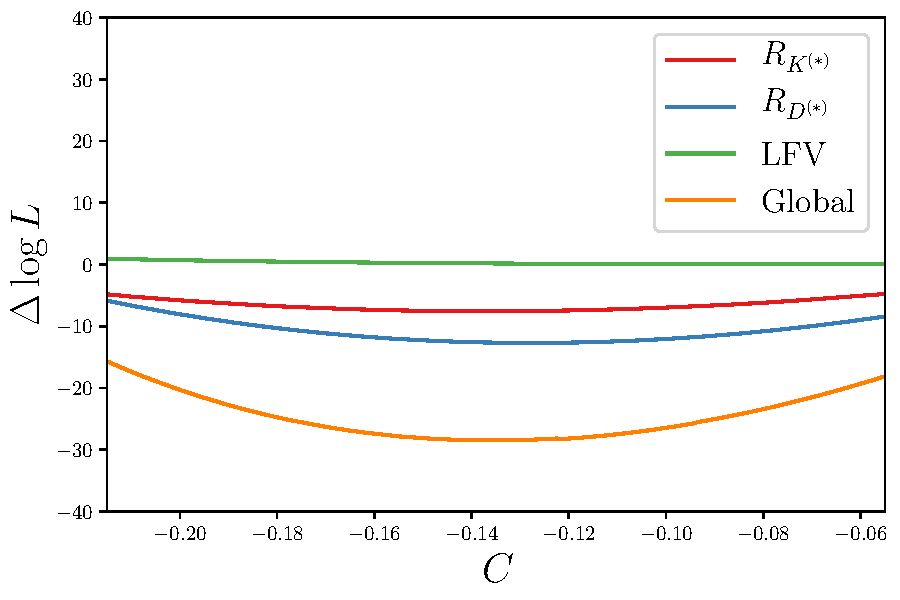
\includegraphics[width=0.19\textwidth]{figures/evoplot_C.pdf}
        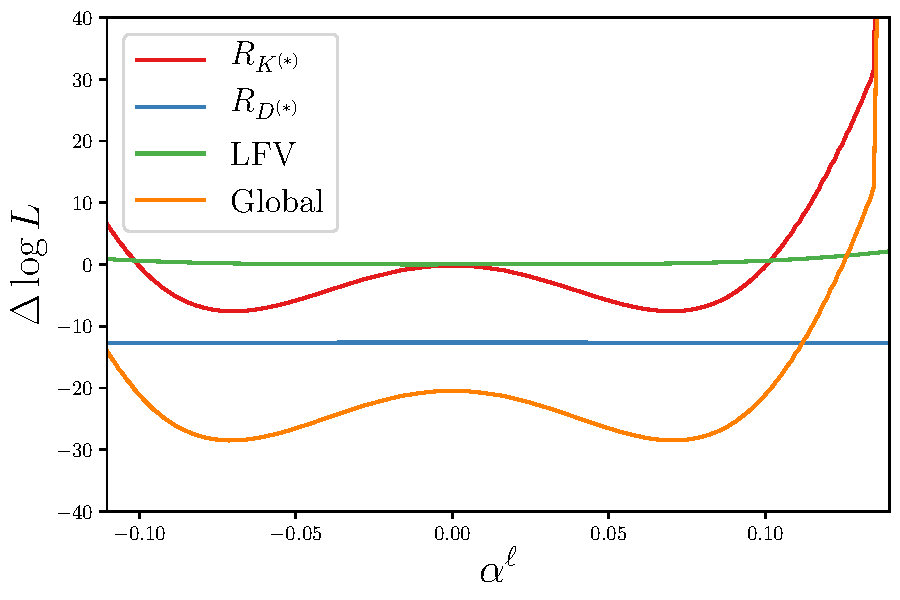
\includegraphics[width=0.19\textwidth]{figures/evoplot_alphal.pdf}
        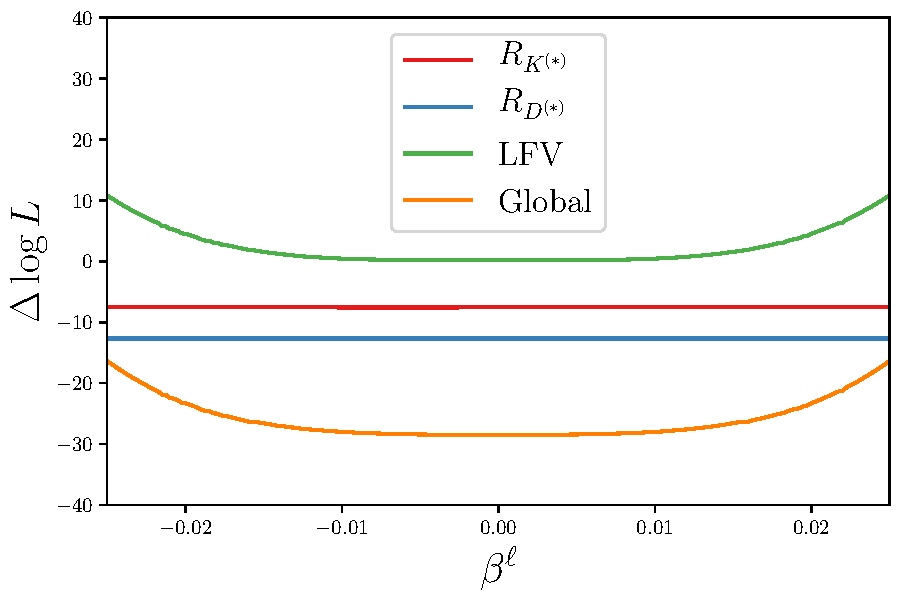
\includegraphics[width=0.19\textwidth]{figures/evoplot_betal.pdf}
        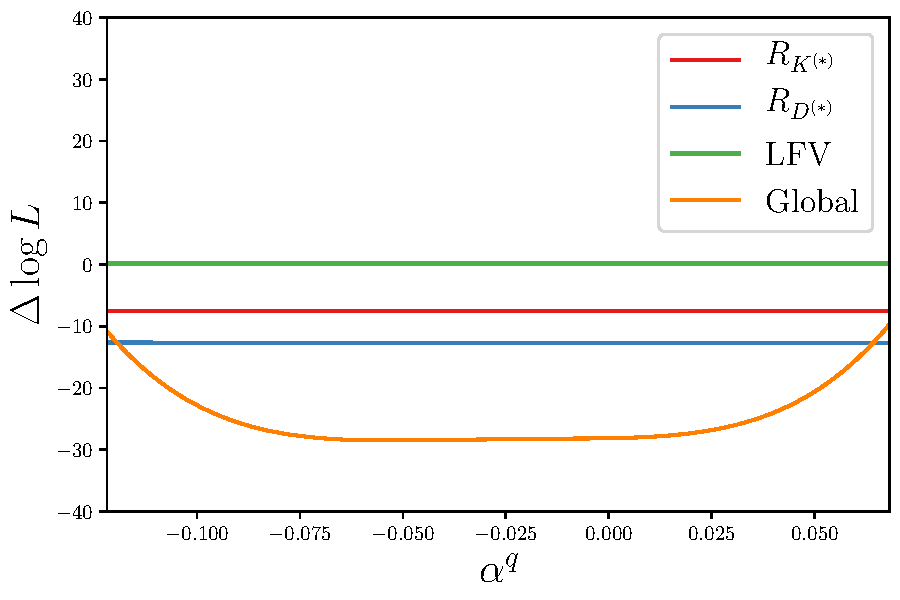
\includegraphics[width=0.19\textwidth]{figures/evoplot_alphaq.pdf}
        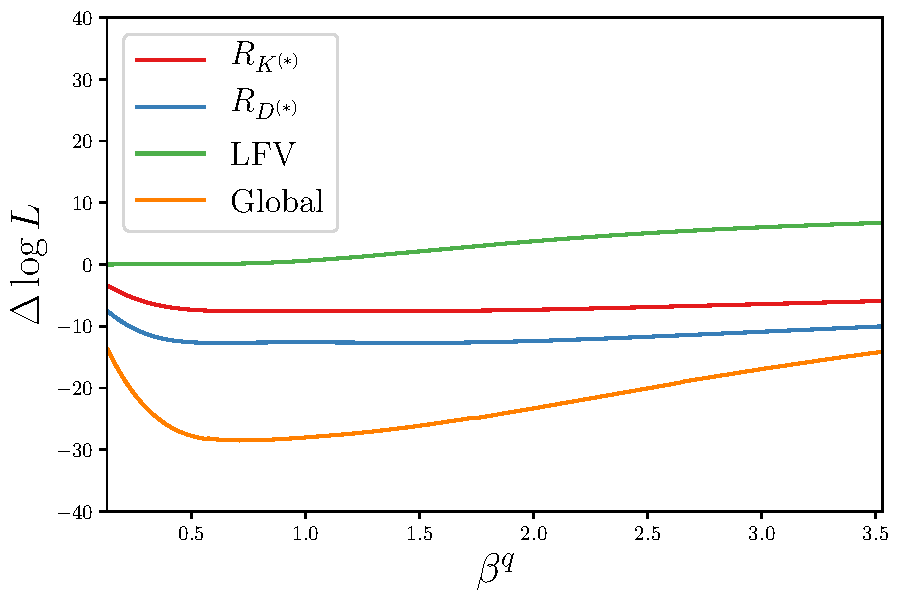
\includegraphics[width=0.19\textwidth]{figures/evoplot_betaq.pdf}
    \end{center}
    \begin{center}
        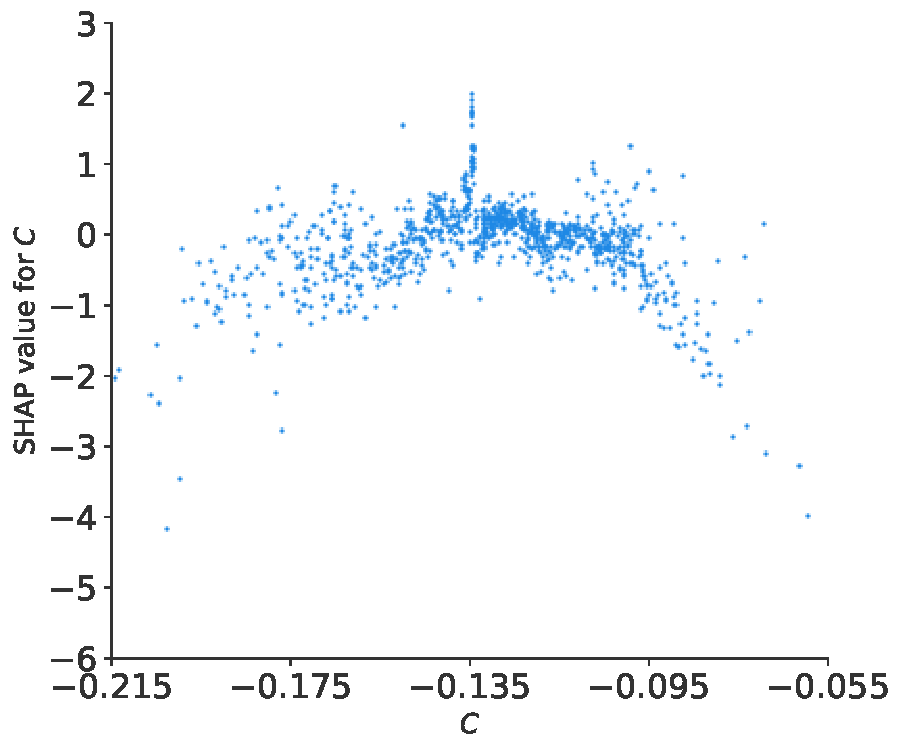
\includegraphics[width=0.19\textwidth]{figures/SHAP_C.pdf}
        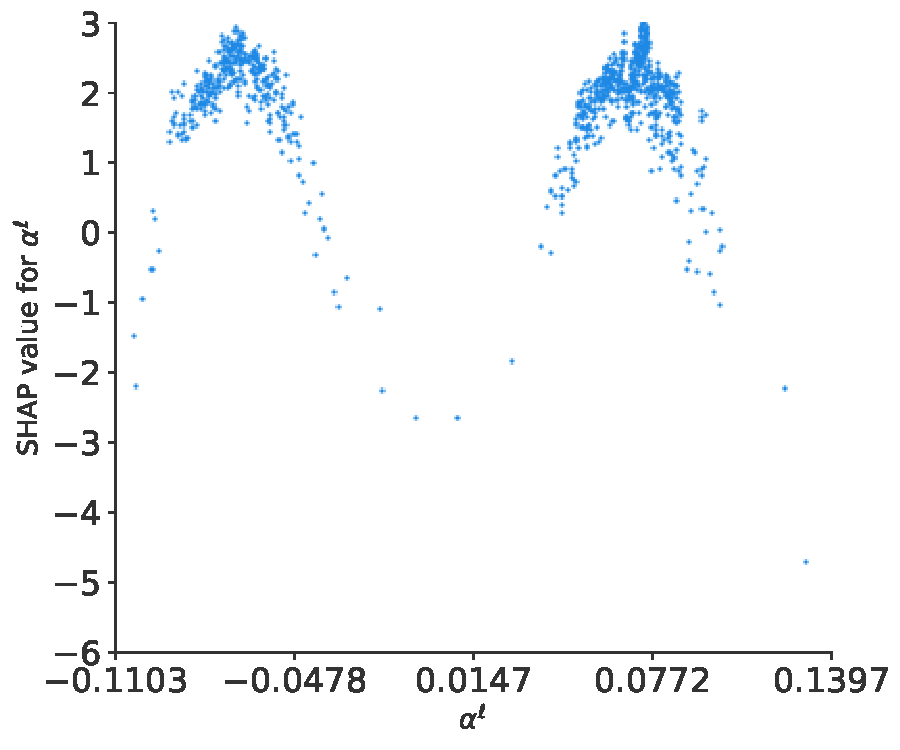
\includegraphics[width=0.19\textwidth]{figures/SHAP_al.pdf}
        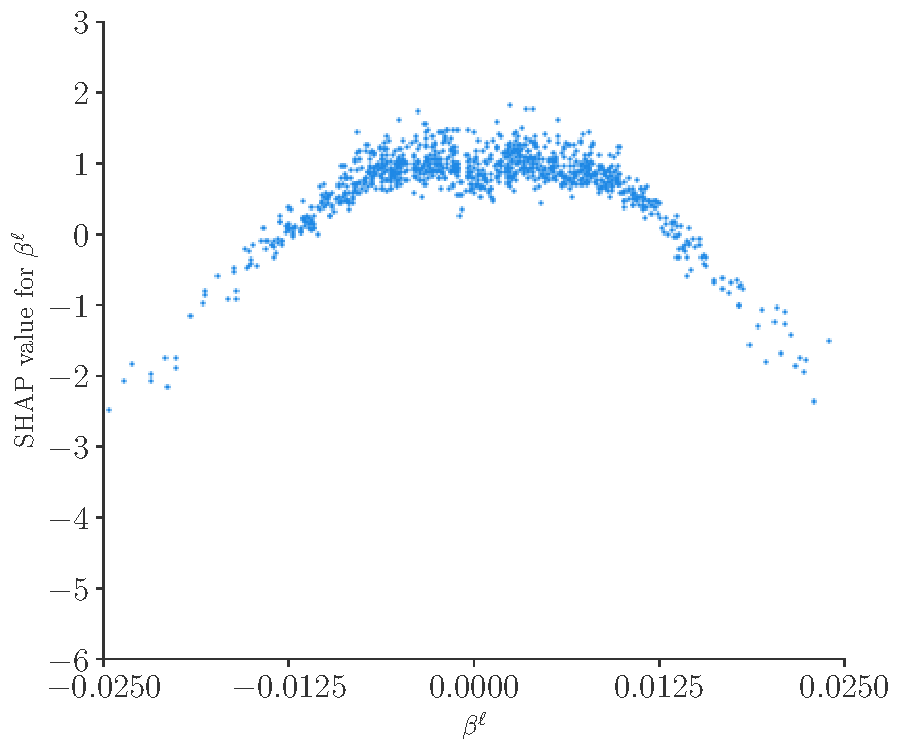
\includegraphics[width=0.19\textwidth]{figures/SHAP_bl.pdf}
        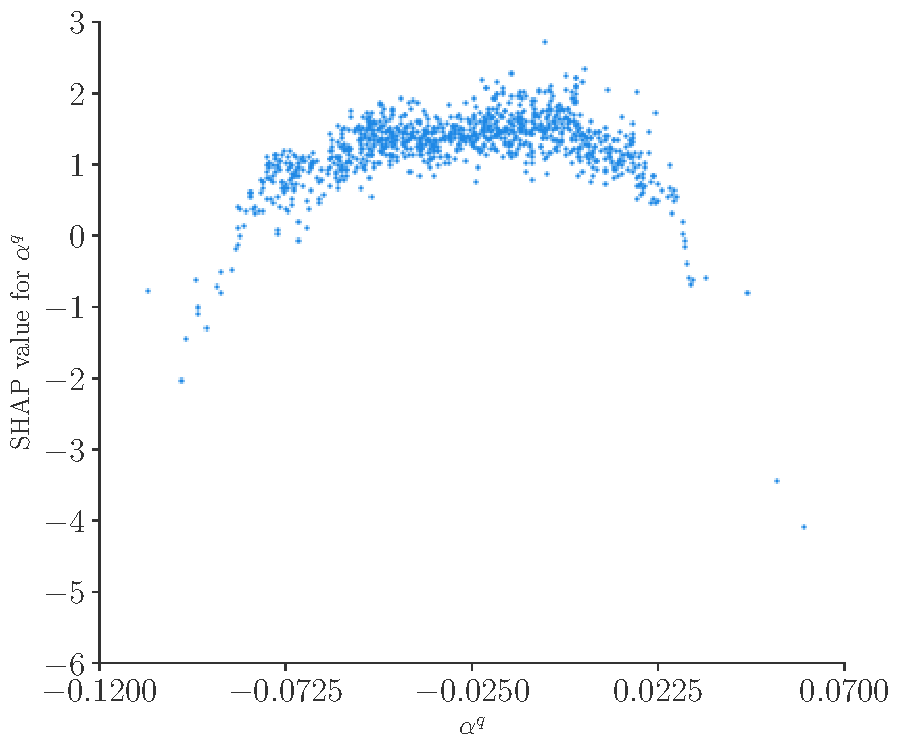
\includegraphics[width=0.19\textwidth]{figures/SHAP_aq.pdf}
        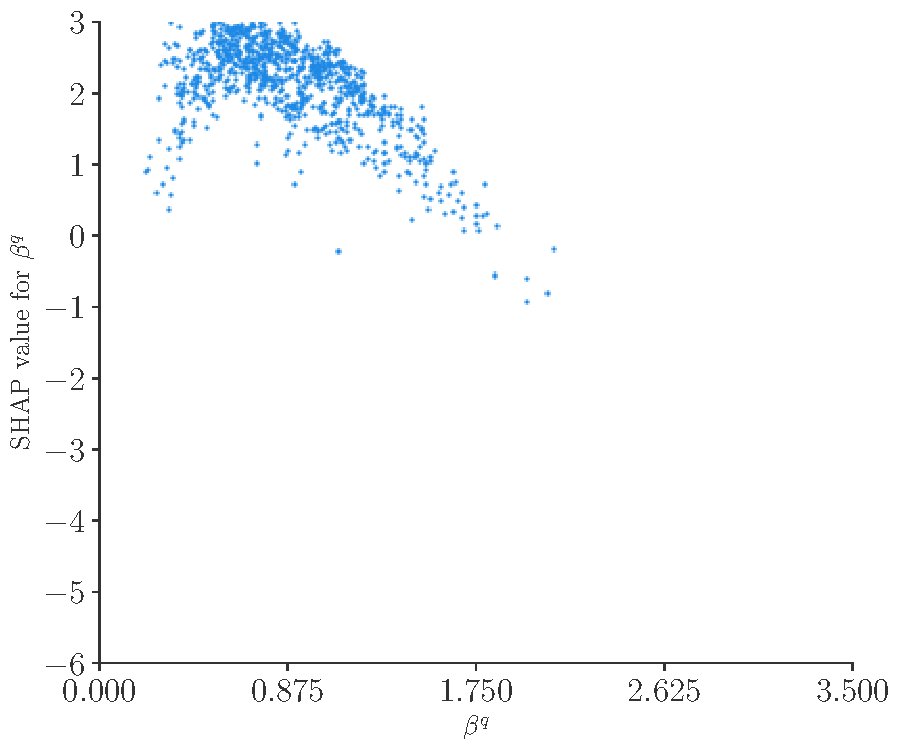
\includegraphics[width=0.19\textwidth]{figures/SHAP_bq.pdf}
    \end{center}
    
    \blankfootnote{\textbf{J.A.}, J. Guasch and S. Peñaranda. arXiv:2109.07404}

\end{frame}

\begin{frame}
    \frametitle{Correlations between WCs}

    \begin{columns}
        \begin{column}{0.5\textwidth}
            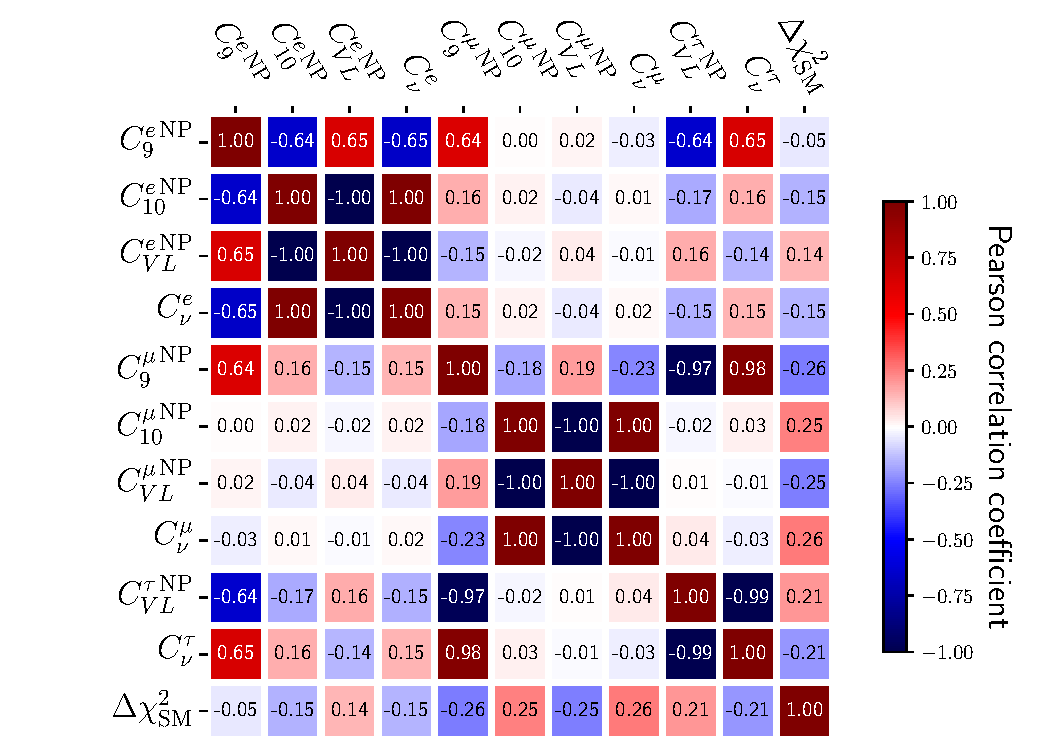
\includegraphics[width=\columnwidth]{figures/coeffcorr.pdf}
        \end{column}
        \begin{column}{0.5\textwidth}
            \begin{itemize}
                \item Correlation in $C_{10}^e$, $C_{VL}^e$ and $C_\nu^e$, all proportional to $C \lambda^q_{23} \lambda^\ell_{11}$.
                \item Correlation in $C_{10}^\mu$, $C_{VL}^\mu$ and $C_\nu^\mu$, all proportional to $C \lambda^q_{23} \lambda^\ell_{22}$.
                \item Correlation in $C_{VL}^\tau$ and $C_\nu^\tau$, all proportional to $C \lambda^q_{23} \lambda^\ell_{33}$.
                \item $C_9^\mu = C_9^\mathrm{loop}$ correlated to $\tau$ sector ($C\lambda^q_{23} \approx C\lambda^q_{23} \lambda^\ell_{33}$).
                \item $C_9^e = -C_{10}^e + C_9^\mathrm{loop}$ partially correlated to $e$ and $\tau$ sectors.
            \end{itemize}
            
        \end{column}
    \end{columns}
    \blankfootnote{\textbf{J.A.}, J. Guasch and S. Peñaranda. arXiv:2109.07404}

\end{frame}

\begin{frame}
    \frametitle{Correlations between observables}

    \begin{columns}
        \begin{column}{0.5\textwidth}
            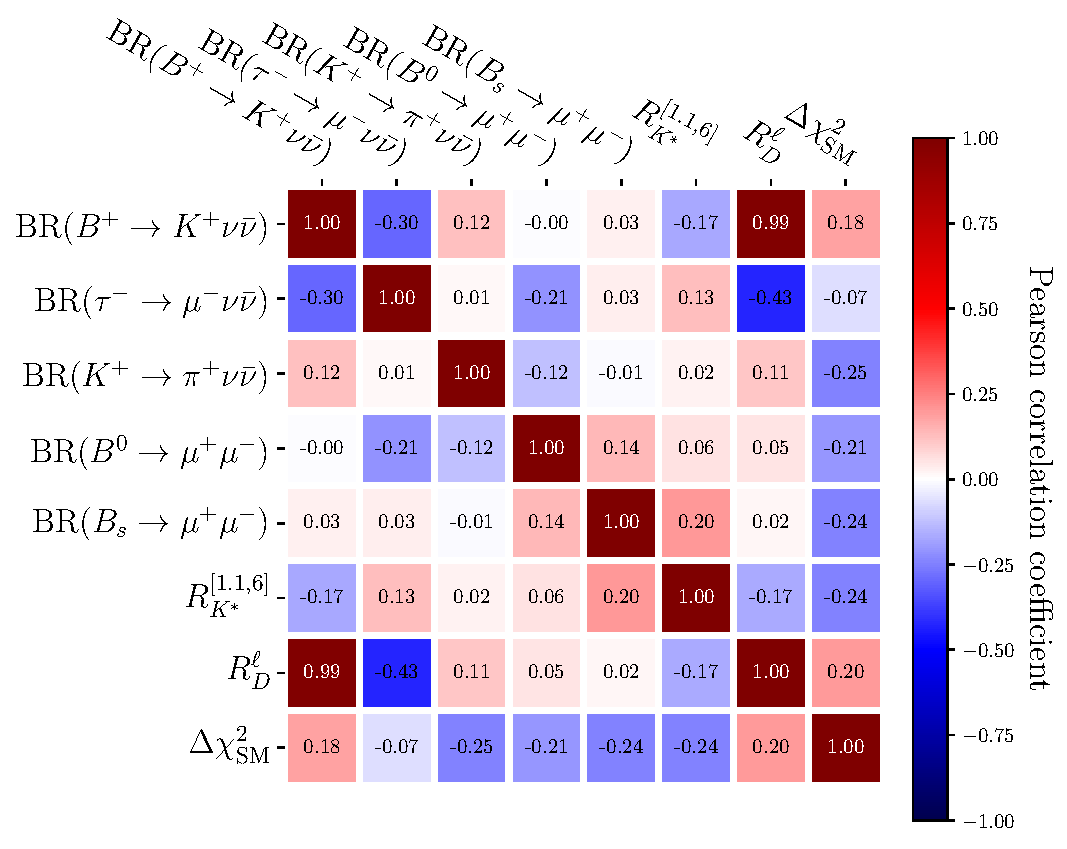
\includegraphics[width=\columnwidth]{figures/obscorr.pdf}
        \end{column}
        \begin{column}{0.5\textwidth}
            \begin{itemize}
                \item Moderate correlation between $R_K$ and $\mathrm{BR}(B_s \to \mu^+ \mu^-)$ because $C_9^\mu \neq C_{10}^\mu$.
                \item Also moderate correlation between $R_K$ and $R_D$.
                \item Perfect correlation between $R_D$ and $\mathrm{BR}(B\to K^{(*)}\nu\bar{\nu})$.
                \item No observable displays large correlations to the global likelihood: global fits are needed.
            \end{itemize}
        \end{column}
    \end{columns}
    \blankfootnote{\textbf{J.A.}, J. Guasch and S. Peñaranda. arXiv:2109.07404}

\end{frame}

\begin{frame}
    \frametitle{$R_D$ and $\mathrm{BR}(B\to K^{(*)}\nu\bar{\nu})$}

    \begin{center}
        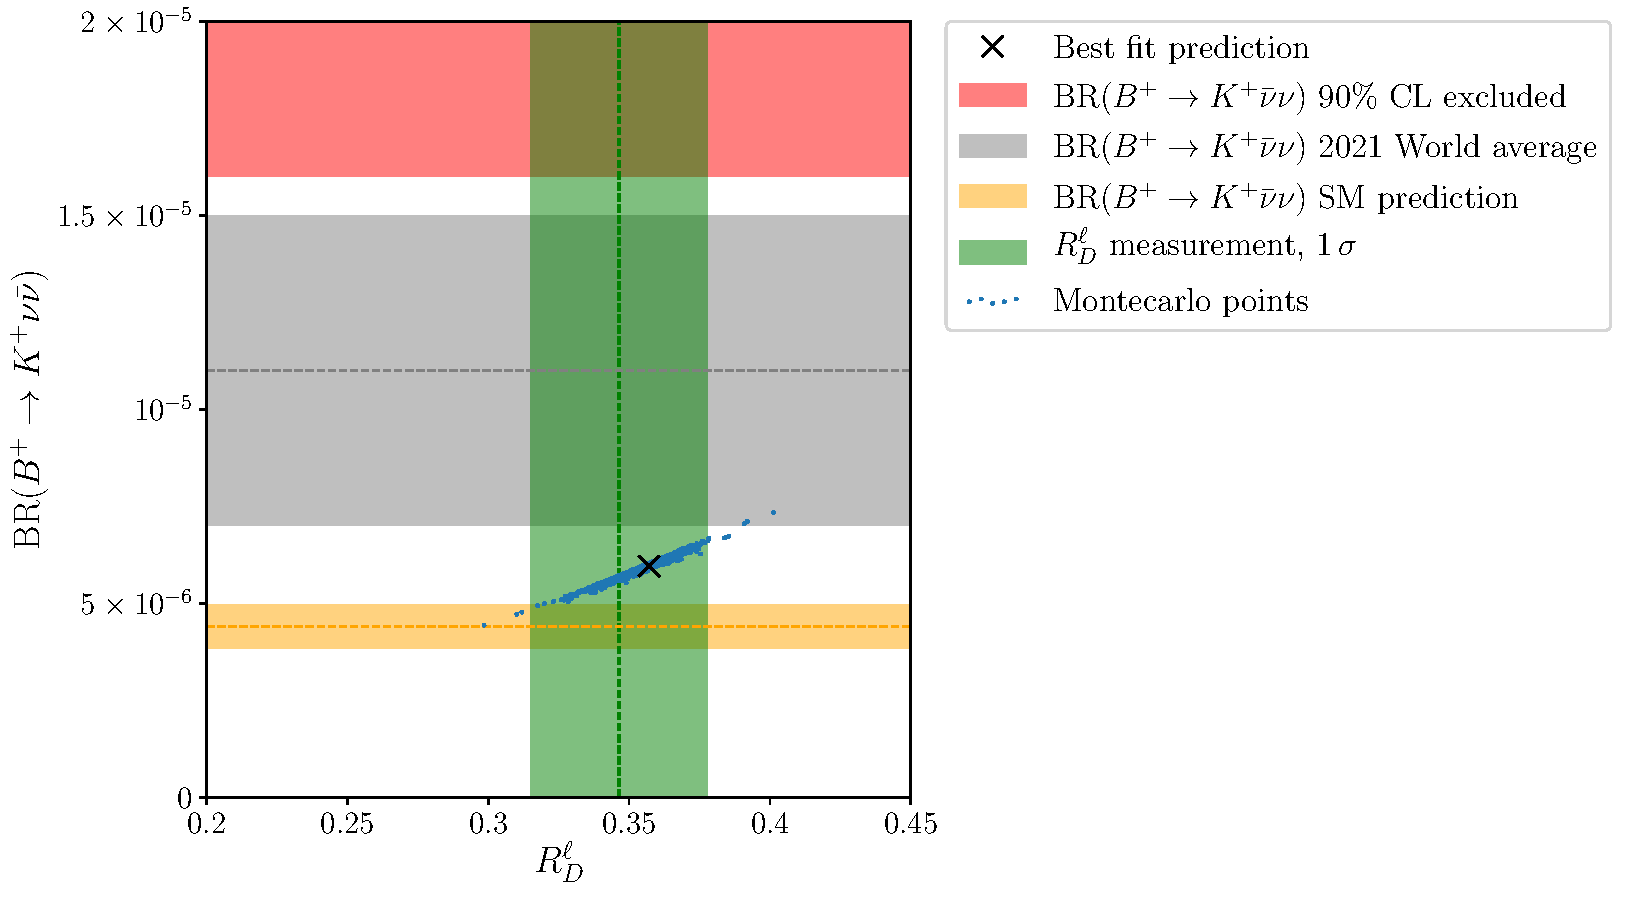
\includegraphics[width=0.8\textwidth]{figures/RD_BKnunu.pdf}
    \end{center}

    An excess in $R_D$ implies an excess in $\mathrm{BR}(B\to K^{(*)}\nu\bar{\nu})$. \\(Note that the {\color{gray}2021 World Average} is not included in our fit).

    \blankfootnote{J. Grygier \textit{et al.} (Belle) arXiv:1702.03224; F. Dattola (Belle-II) arXiv:2105.05754; Y. S. Ahmis \textit{et al.} (HFLAV) arXiv:1909.12524; \textbf{J.A.}, J. Guasch and S. Peñaranda. arXiv:2109.07404}
\end{frame}


\begin{frame}
    \frametitle{Connection to Leptoquarks}

    Vector Leptoquark $U_1 \sim (\bar{\mathbf{3}}, \mathbf{1}, 2/3)$,
    $$\mathcal{L}_{U_1} = x_L^{ij} \bar{q}_i \gamma_\mu U_1^\mu \ell_j + x_R^{ij} \bar{d}_{Ri} \gamma_\mu U_1^\mu e_{Rj} + \mathrm{h.c.} $$

    Matching to the SMEFT Wilson coefficients
    $$C_{\ell q(1)}^{ijkl} = C_{\ell q(3)}^{ijkl} = \frac{-\Lambda^2}{2M_U^2}x_L^{li}x_L^{kj*}\,,$$
    $$C_{ed}^{ijkl} = -\frac{1}{2}C_{qde}^{ijkl} = \frac{-\Lambda^2}{2M_U^2}x_R^{li}x_R^{kj*}\,,$$
    In terms of the parameters of our fit,
    $$|x_L^{ji}|^2 = -\frac{2}{M_U^2}C\lambda^\ell_{ii}\lambda^q_{jj}\,,$$
    $$\mathrm{Arg}(x_L^{ji}) = \mathrm{Arg}(\lambda_{j3}^q)-\mathrm{Arg}(\lambda_{i3}^\ell) + \theta\,.$$ % chktex 21

\end{frame}

\begin{frame}
    \frametitle{Connection to leptoquarks}

    $$x_L = \begin{pmatrix}
        -2.27\times10^{-3} & -3.76\times 10^{-10}  & -0.0325 \\
        0.0319 & 5.29\times 10^{-9} &  0.458\\
        0.0437  & 7.25\times 10^{-9}  & 0.627
        \end{pmatrix}\,.
    $$
    \begin{itemize}
        \item Couplings $x_L^{23}$ and $x_L^{33}$, previously proposed to describe the $R_{D^{(*)}}$ anomaly\footnote[1]{A.~Bhaskar, D.~Das, T.~Mandal, S.~Mitra and C.~Neeraj. 2101.12069}. Compatible with experimental limits.
        \item Additionally, couplings $x_L^{21}$ and $x_L^{31}$ to describe the $R_{K^{(*)}}$ anomaly. 
    \end{itemize}

    ~
    
    Other leptoquark models, and $W'$ and $Z'$ models, do not generate $C_{\ell q(1)} = C_{\ell q (3)}$. 
\end{frame}

\begin{frame}
    \frametitle{Conclusions}

    \begin{itemize}
        \item Using EFTs (SMEFT) to describe the $R_{K^{(*)}}$ and $R_{D^{(*)}}$ anomalies: $R_{D^{(*)}}$ generated at tree level and $R_{K^{(*)}}$ from interplay between tree and loop level.
        \item Global fits are needed to take in account possible side-effects. 
        \item \texttt{xgboost} Machine Learning model is able to approximate the likelihood function.
        \item SHAP values capture the importance of each parameter in the fit.
        \item Interesting correlation between $R_{D^{(*)}}$ and $\mathrm{BR}(B\to K^{(*)}\nu\bar{\nu})$.
        \item Explanation in terms of vector leptoquark $U_1$ coupling to second and third generations of quarks and third ($R_{D^{(*)}}$) and first ($R_{K^{(*)}}$) generation of leptons.
    \end{itemize}

\end{frame}

\end{document} %chktex 17